%%%%%%%%%%%%%%%%%%%%%%%%%%%%%%%%%%%%%%%%%
% Beamer Presentation
% LaTeX Template
% Version 1.0 (10/11/12)
%
% This template has been downloaded from:
% http://www.LaTeXTemplates.com
%
% License:
% CC BY-NC-SA 3.0 (http://creativecommons.org/licenses/by-nc-sa/3.0/)
%
%%%%%%%%%%%%%%%%%%%%%%%%%%%%%%%%%%%%%%%%%

%----------------------------------------------------------------------------------------
%	PACKAGES AND THEMES
%----------------------------------------------------------------------------------------

\documentclass{beamer}

\mode<presentation> {

% The Beamer class comes with a number of default slide themes
% which change the colors and layouts of slides. Below this is a list
% of all the themes, uncomment each in turn to see what they look like.

%\usetheme{default}
%\usetheme{AnnArbor}
%\usetheme{Antibes}
%\usetheme{Bergen}
%\usetheme{Berkeley}
%\usetheme{Berlin}
%\usetheme{Boadilla}
%\usetheme{CambridgeUS}
%\usetheme{Copenhagen}
%\usetheme{Darmstadt}
%\usetheme{Dresden}
%\usetheme{Frankfurt}
%\usetheme{Goettingen}
%\usetheme{Hannover}
%\usetheme{Ilmenau}
%\usetheme{JuanLesPins}
%\usetheme{Luebeck}
\usetheme{Madrid}
%\usetheme{Malmoe}
%\usetheme{Marburg}
%\usetheme{Montpellier}
%\usetheme{PaloAlto}
%\usetheme{Pittsburgh}
%\usetheme{Rochester}
%\usetheme{Singapore}
%\usetheme{Szeged}
%\usetheme{Warsaw}

% As well as themes, the Beamer class has a number of color themes
% for any slide theme. Uncomment each of these in turn to see how it
% changes the colors of your current slide theme.

%\usecolortheme{albatross}
%\usecolortheme{beaver}
%\usecolortheme{beetle}
%\usecolortheme{crane}
%\usecolortheme{dolphin}
%\usecolortheme{dove}
%\usecolortheme{fly}
%\usecolortheme{lily}
%\usecolortheme{orchid}
%\usecolortheme{rose}
%\usecolortheme{seagull}
%\usecolortheme{seahorse}
%\usecolortheme{whale}
%\usecolortheme{wolverine}

\usefonttheme{serif} 

%\setbeamertemplate{footline} % To remove the footer line in all slides uncomment this line
%\setbeamertemplate{footline}[page number] % To replace the footer line in all slides with a simple slide count uncomment this line

\setbeamertemplate{navigation symbols}{} % To remove the navigation symbols from the bottom of all slides uncomment this line
}

\usepackage{graphicx} % Allows including images
\usepackage{booktabs} % Allows the use of \toprule, \midrule and \bottomrule in tables
\usepackage[T1]{fontenc}
\usepackage[utf8]{inputenc}
\usepackage{amsmath}
\usepackage{color}
\usepackage[czech]{babel}
\usepackage{lmodern}  
\usepackage{rotating}
\usepackage{scrextend}
\usepackage{pifont}
\usepackage{hyperref}
\usepackage{bm}

%----------------------------------------------------------------------------------------
%	TITLE PAGE
%----------------------------------------------------------------------------------------

\title[Týden 4]{Praktikum z ekonometrie - Týden 4} % The short title appears at the bottom of every slide, the full title is only on the title page

\author{VŠE Praha} % Your name
\institute[4EK417] % Your institution as it will appear on the bottom of every slide, may be shorthand to save space
{
% Your institution for the title page
\medskip
\textit{Tomáš Formánek} % Your email address
}
\date{} % Date, can be changed to a custom date

\begin{document}

\begin{frame}
\titlepage % Print the title page as the first slide
\end{frame}

\begin{frame}
\frametitle{Outline} % Table of contents slide, comment this block out to remove it
\tableofcontents % Throughout your presentation, if you choose to use \section{} and \subsection{} commands, these will automatically be printed on this slide as an overview of your presentation
\end{frame}

%----------------------------------------------------------------------------------------
%	PRESENTATION SLIDES
%---------------------------------------------------------------------
\begin{frame}{Introduction}

\begin{itemize}
\item \textbf{Subset Selection} We identify a subset of the $p$ predictors
that we believe to be related to the response. We then fit a
model using least squares on the reduced set of variables.
\medskip
\item \textbf{Shrinkage} We fit a model involving all $p$ predictors, but
the estimated coefficients are shrunken towards zero
relative to the least squares estimates. This shrinkage (also
known as regularization) has the effect of reducing variance
and can also perform variable selection.
\medskip
\item \textbf{Dimension Reduction} We project the $p$ predictors into a
$M$-dimensional subspace, where $M < p$. This is achieved by
computing $M$ different linear combinations, or projections,
of the variables. Then these $M$ projections are used as
predictors to fit \\a linear regression model by least squares.

\end{itemize}

\end{frame}





%----------------------------------------------------------------------------------------
\section{Model selection algorithms} % Sections can be created in order to organize your presentation into discrete blocks, all sections and subsections are automatically printed in the table of contents as an overview of the talk
%------------------------------------------------

% \subsection{} % A subsection can be created just before a set of slides with a common theme to further break down your presentation into chunks
%------------------------------------------------

\begin{frame}
\frametitle{Model selection algorithms}

\begin{enumerate}
  \item Best subset selection
  \medskip
  \item Forward stepwise selection
  \medskip
  \item Backward stepwise selection
  \medskip
  \item Algorithms combining Forward and Backward stepwise selection\\
  ~\\
 (Comparison \& computational complexity of methods)
\end{enumerate}


\end{frame}

%------------------------------------------------
\subsection{Best subset selection}
\begin{frame}
\frametitle{Best subset selection}

\begin{enumerate}
  \item Let $\mathcal{M}_0$ denote the \textit{null model}, which contains no predictors.
  \\Say, $y_i=\beta_0+u_i$
  \\ This model simply predicts the sample mean for $y$.
  \item For $k= 1,2, \dots ,p$:
  \begin{enumerate}[{(a)}]
  \item Fit all $\binom{p}{k}$ models that contain exactly $k$ predictors.
  \item Choose the best among these $\binom{p}{k}$ models and call it $\mathcal{M}_{k}$.
        \\Here, best is defined as having smallest $\textit{RSS}$ or highest $R^2$.
\end{enumerate}
  \item Select a single best model from among $\mathcal{M}_0, \dots, \mathcal{M}_{p}$, using crossvalidated prediction error, $\textit{AIC}, \textit{BIC}$ or adjusted $R^2$.

\vspace{0.8cm}

\item[] Note: $\binom{p}{k}=\frac{p!}{k!(p-k)!}$ \hspace{0.5cm}; \hspace{0.5cm} $\sum_{k=1}^p \binom{p}{k} = 2^p$

\end{enumerate}
\end{frame}


%------------------------------------------------
\subsection{Forward stepwise selection}
\begin{frame}
\frametitle{Forward stepwise selection}

\begin{enumerate}
  \item Let $\mathcal{M}_0$ denote the \textit{null model}, which contains no predictors.
  \\Say, $y_i=\beta_0+u_i$
  \item For $k=0,1, \dots , \left(p-1\right)$:
\begin{enumerate}[{(a)}]
  \item Consider all $(p-k)$ models that augment the predictors in $\mathcal{M}_k$ with one additional predictor.
  \item Choose the best among these $(p-k)$ models, and call it $\mathcal{M}_{k+1}$.
        \\Here, best is defined as having smallest $\textit{RSS}$ or highest $R^2$.
\end{enumerate}
  \item Select a single best model from among $\mathcal{M}_0, \dots, \mathcal{M}_{p}$, using crossvalidated
prediction error, $\textit{AIC}, \textit{BIC}$ or adjusted $R^2$.
\end{enumerate}

\end{frame}

%------------------------------------------------
\subsection{Backward stepwise selection}
\begin{frame}
\frametitle{Backward stepwise selection}

\begin{enumerate}
  \item Let $\mathcal{M}_p$ denote the \textit{full model}, which contains all $p$ predictors.
  \\Say, $y_i=\beta_0+ \beta_1x_{i1} + \dots + \beta_px_{ip} + u_i$
  \item For $k=p, (p-1), \dots , 1$:
\begin{enumerate}[{(a)}]
  \item Consider all $k$ models that contain all but one of the predictors
in $\mathcal{M}_k$, for a total of $(k-1)$ predictors.
  \item Choose the best among these $k$ models, and call it $\mathcal{M}_{k-1}$.
        \\Here, best is defined as having smallest $\textit{RSS}$ or highest $R^2$.
\end{enumerate}
  \item Select a single best model from among $\mathcal{M}_0, \dots, \mathcal{M}_{p}$, using crossvalidated
prediction error, $\textit{AIC}, \textit{BIC}$ or adjusted $R^2$.
\end{enumerate}

\end{frame}

%------------------------------------------------

\begin{frame}
\frametitle{Comparison \& computational complexity of methods}
\textbf{Statistics for comparison of models/methods:} 

\begin{equation} \notag
\begin{aligned}
 \textnormal{Mallow's} \hspace{0.2cm}
 \textit{C}_{p} &=\frac{1}{n}(\textit{RSS}+2d\widehat{\sigma}^2), \\
 \smallskip
 \textit{AIC} &=\frac{1}{n\widehat{\sigma}^2}(\textit{RSS}+2d\widehat{\sigma}^2), \\
 \smallskip
 \textit{BIC} &=\frac{1}{n}(\textit{RSS}+log(n)d\widehat{\sigma}^2),
 \end{aligned}
\end{equation}

\begin{itemize}
\item where $d$ is the number of regressors and $n$ is the sample size.
\item Model selection: find a model where a statistic is minimized.
\item $log(n) > 2$ for $n>7$. $\Rightarrow$ $\textit{BIC}$ penalizes model complexity more.
\item $\textit{AIC} \propto C_p$;~~ $\textit{AIC}$ and $\textit{BIC}$ may contradict 
\item If $\widehat{\sigma}^2$ is an unbiased estimate of ${\sigma}^2$, 
\\then $C_p$ is an unbiased estimate of test $\textit{MSE}$.
\end{itemize}
\medskip
\textbf{\textit{k}FCV methods}: $k$-fold cross validation


\end{frame}

%------------------------------------------------

\begin{frame}
\frametitle{Comparison \& computational complexity of methods}

\textbf{Computational complexity:} 
\bigskip
\begin{itemize}
  \item Forward stepwise and Backward stepwise selection
        \\ Greedy algorithms.
        \\$[1+p(p+1)/2] \approx p^2$ models need to be estimated and evaluated.
        \\Computationally feasible even for high $p$ values (large sets of potential regressors).
        \vspace{0.5cm}
  \item Best subset selection
        \\ $2^p$ models to be estimated and evaluated.
        \\ For large $p$, enormous search space can lead to over-fitting and high variance of the coefficient estimates.

\end{itemize}

\bigskip

Forward \& Backward stepwise [and their hybrid combinations] tends to do well in practice (are efficient algorithms), yet they do not guarantee finding the best possible model out of all $2^p$ possible models.
\end{frame}

%------------------------------------------------
\section{Parameter Shrinkage}
\begin{frame}{Parameter shrinkage methods}
\textbf{Ridge regression and Lasso regression}
\medskip
\begin{itemize}
\item As an alternative to stepwise selection, we can fit a model containing all $p$ predictors using a technique that constrains or regularizes the coefficient estimates, or equivalently, that shrinks the coefficient estimates towards zero.
\medskip
\item It may not be immediately obvious why such a constraint
should improve the fit, but it turns out that shrinking the
coefficient estimates can significantly reduce their variance.
\end{itemize}
\end{frame}
%------------------------------------------------
\subsection{Ridge regression}
\begin{frame}{Ridge regression}
Consider a LRM: $y = f( x_1, x_2, \dots , x_p)$

\begin{itemize}
\item \textbf{OLS} can be used to estimate $\bm{\hat{\beta}}=(\hat{\beta}_0, \hat{\beta}_1, \dots , \hat{\beta}_p)^{\prime}$ by minimizing the RSS:
$$ RSS = \sum_{i=1}^n \left(y_i - \hat{\beta}_0 
         - \sum_{j=1}^p  \hat{\beta}_j x_{ij}      \right)^2 $$
\bigskip
\item \textbf{Ridge regression} $\bm{\hat{\beta}}_{\!R}$ estimates 
are the values that minimize:
$$ \sum_{i=1}^n \left(y_i - \hat{\beta}_0 
         - \sum_{j=1}^p  \hat{\beta}_j x_{ij} \right)^2 
         \! + \lambda \sum_{j=1}^p  \hat{\beta}_j^2
         \, = \, RSS + \lambda \sum_{j=1}^p  \hat{\beta}_j^2 ,$$
where $\lambda > 0$ is a tuning parameter, determined separately.
\end{itemize}
\end{frame}
%------------------------------------------------
\begin{frame}{Ridge regression}
\begin{itemize}
\item As with least squares, ridge regression seeks coefficient estimates that fit the data well, by making the RSS small.
\medskip
\item However, the second term, $\, \lambda \sum_{j=1}^p  \hat{\beta}_j^2 \,$, called a shrinkage penalty, is small when $\hat{\beta}_1, \dots, \hat{\beta}_p$ are close to zero. Hence, $\lambda$ has the effect of shrinking $\hat{\beta}_j^2$ towards zero.
\medskip
\item The tuning parameter $\lambda$ serves to control the relative impact of the two terms on the regression coefficient estimates.
\medskip
\item Selecting a good value for $\lambda$ is critical; cross-validation is used.
\end{itemize}
\end{frame}
%------------------------------------------------
\begin{frame}{Ridge regression - example}
\vspace{-1cm}
\begin{figure}
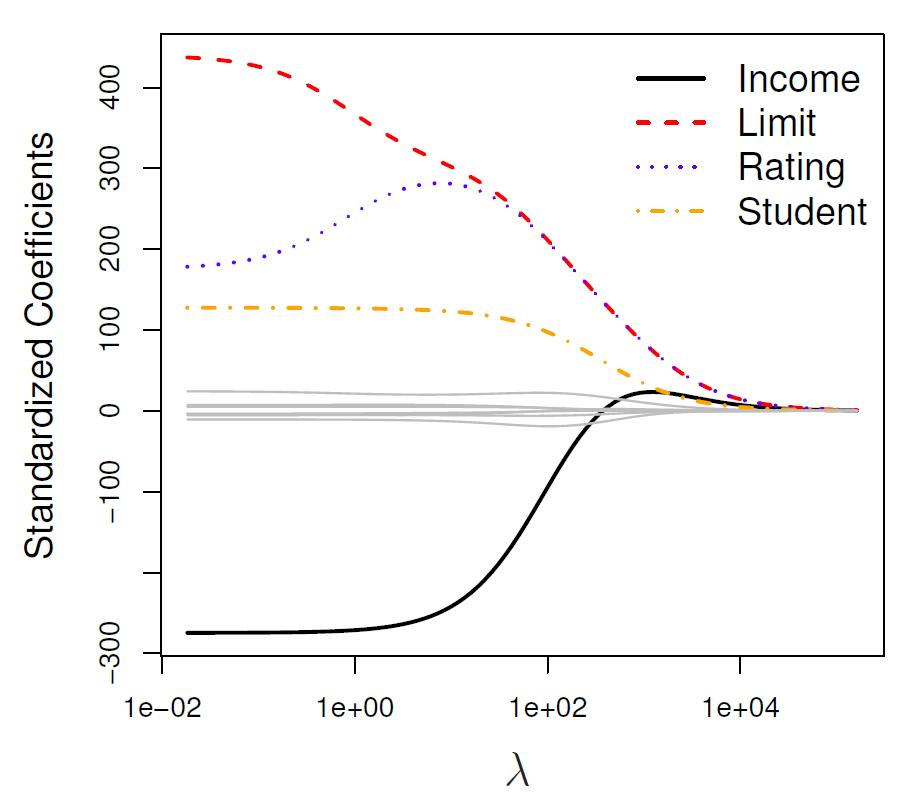
\includegraphics[scale=0.30]{IMG/Ridge.jpg}
\end{figure}
\vspace{-0.5cm}
\centering Coefficient estimates are plotted as a function of $\lambda$.
\end{frame}

%------------------------------------------------
\begin{frame}{Ridge regression}
\begin{itemize}
\item The standard least squares coefficient estimates are scale
equivariant: multiplying $x_j$ by a constant $c$ simply leads to
a scaling of the least squares coefficient estimates by a
factor of $1/c$.\\ 
\medskip Regardless of $j$-th
predictor scaling, $ \hat{\beta}_j x_{ij}$ will remain the same.
\medskip
\item In contrast, the ridge regression coefficient estimates can
change substantially when multiplying a given predictor by
a constant, due to the sum of squared coefficients term in
the penalty part of the ridge regression objective function.
\medskip
\item Therefore, it is best to apply ridge regression after
standardizing the predictors, using the formula:

$$ \widetilde{x}_{ij} = \frac{x_{ij}}{
   \sqrt[]{\frac{1}{n} \sum_{i=1}^n (x_{ij} - \overline{x}_j)^2 \,   }}$$
 
\end{itemize}
\end{frame}
%------------------------------------------------
\subsection{Lasso regression}
\begin{frame}{Lasso regression}
\begin{itemize}
\item Ridge regression does have one obvious disadvantage:
unlike subset selection, which will generally select models
that involve just a subset of the variables, ridge regression
will include all $p$ predictors in the final model.
\medskip
\item The Lasso is a relatively recent alternative to ridge
regression that overcomes this disadvantage. The lasso
coefficients,  $\bm{\hat{\beta}}_{\!L}$ estimates 
are the values that minimize:
$$ \sum_{i=1}^n \left(y_i - \hat{\beta}_0 
         - \sum_{j=1}^p  \hat{\beta}_j x_{ij} \right)^2 
         \! + \lambda \sum_{j=1}^p  | \hat{\beta}_j |
         \, = \, RSS + \lambda \sum_{j=1}^p  | \hat{\beta}_j |,$$
again, $\lambda > 0$ is a tuning parameter, determined separately ($k$FCV).
\item In statistical parlance, the lasso uses an $\ell_1$ (pronounced ``ell 1'') penalty instead of an $\ell_2$ penalty. The $\ell_1$ norm of a coefficient vector  is given by 
$\| \beta \|_1 = \sum | \beta |$.
\end{itemize}
\end{frame}
%------------------------------------------------
\begin{frame}{Lasso regression - example}
\vspace{-1cm}
\begin{figure}
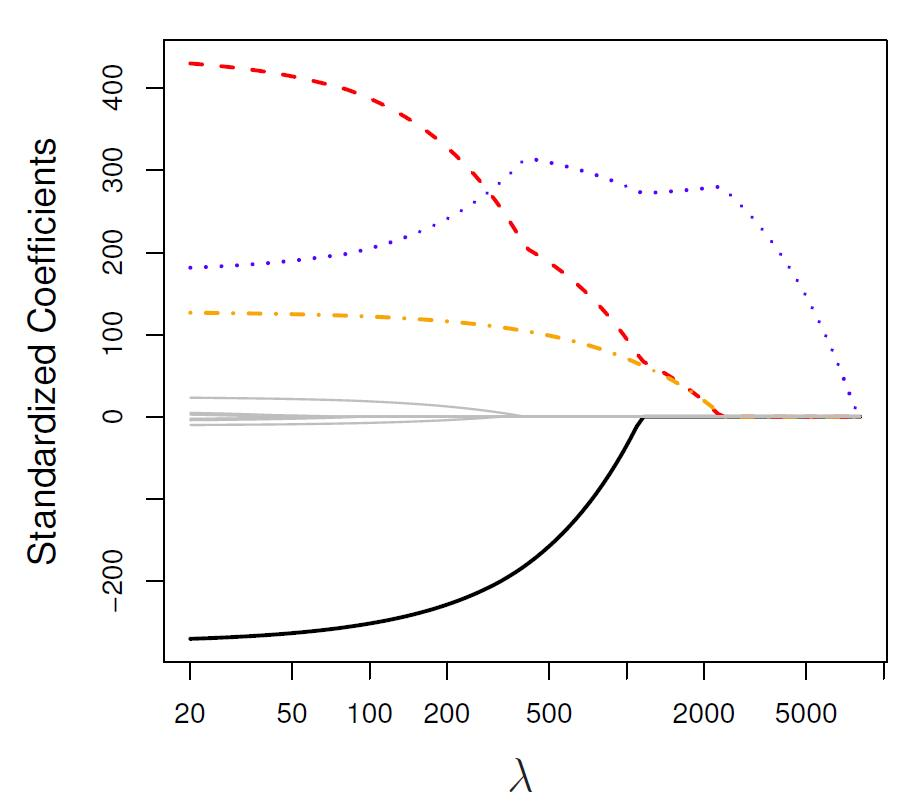
\includegraphics[scale=0.30]{IMG/Lasso.jpg}
\end{figure}
\vspace{-0.5cm}
\centering Coefficient estimates are plotted as a function of $\lambda$.
\end{frame}
%------------------------------------------------
\begin{frame}{Lasso regression}
\begin{itemize}
\item As with ridge regression, the lasso shrinks the coefficient
estimates towards zero.
\medskip
\item In the case of the lasso, the $\ell_1$ penalty has the
effect of forcing some of the coefficient estimates to be
exactly equal to zero when the tuning parameter $\lambda$ is
sufficiently large (see \textcolor{blue}{\underline{\href{http://www-bcf.usc.edu/~gareth/ISL/}{ISLR textbook}}})
\medskip
\item Much like best subset selection, the lasso performs
variable selection.
\medskip
\item Lasso yields sparse models - that is, models that involve only a subset of the variables.
\medskip
\item As in ridge regression, selecting a good value of $\lambda$ for the
lasso is critical; cross-validation is used.
\end{itemize}
\end{frame}
%------------------------------------------------
\begin{frame}{Ridge \& Lasso - discussion}
\begin{itemize}
\item Neither ridge regression nor the lasso will universally dominate the other.
\medskip
\item In general, one might expect the lasso to perform better
when the response is a function of only a relatively small
number of predictors.
\medskip
\item However, the number of predictors that is related to the
response is never known a priori for real data sets.
\medskip
\item Cross-validation can be used in order to determine which approach is better on a particular data set.
\end{itemize}
\end{frame}
%------------------------------------------------
\begin{frame}{Ridge \& Lasso - $\lambda$ selection}

Cross-validation is used to determine $\lambda$, as follows:
\bigskip
\begin{enumerate}
\item We choose a grid of $\lambda$ values and compute the
cross-validation error rate for each value of $\lambda$.
\medskip
\item We select the tuning parameter $\lambda$, for which the
cross-validation error is smallest.
\medskip
\item Finally, the model is re-fit using all of the available
observations and the selected value of the tuning
parameter $\lambda$.
\end{enumerate}
\bigskip
The above steps 1 and 2 can be performed for both ridge and lasso.\\
~~\dots cross-validation errors are compared to select ``best'' $\lambda$ \\
~~\dots and to chose between ridge and lasso.

\end{frame}
%------------------------------------------------
\section{Dimension Reduction}
\begin{frame}{Dimension reduction methods}
\begin{itemize}
\item Stepwise regression, ridge and lasso involve fitting linear regression models (by OLS or by parameter shrinkage) using the original predictors $X_1, X_2, \dots , X_p$.
\medskip
\item \textbf{Dimension reduction methods} transform the
predictors and then fit a least squares model using the
transformed variables:
\begin{enumerate}
\bigskip
\item \textbf{Principal components analysis} is used for data pre-processing, before supervised techniques are applied (dimension reduction).
\bigskip
\item \textbf{Principal component regression}:  In the LRM, the potentially many correlated original variables are replaced with a small set of principal components that capture their joint variation.
\end{enumerate}
\end{itemize}
\end{frame}
%------------------------------------------------
\subsection{Principal component analysis (PCA)}
\begin{frame}{Principal component analysis (PCA)}
\begin{itemize}
\item PCA produces a low-dimensional representation of a dataset. It finds a sequence of linear combinations of the variables that have maximal variance and are mutually uncorrelated.
\bigskip
\item Apart from producing derived variables for use in supervised learning problems, PCA also serves as a tool for data visualization.
\medskip
\item Suppose we have a $(n \! \times \! p)$ dataset $\bm{X}$. Since we are mainly interested in variance here, we can assume that each of the variables in $\bm{X}$ has been \textbf{centered} to have mean zero (all column means of $\bm{X}$ are zero).\\
\medskip
If necessary, the transformation (centering) is straight-forward.

\end{itemize}
\end{frame}
%----------------------------------------------------------------------
\begin{frame}{Principal component analysis (PCA)}
\begin{itemize}
\item The \textbf{first principal component} of a set of centered variables
$X_1, X_2, \dots, X_p$ is the normalized linear combination:
$$ Z_1 = \phi_{11}X_1 + \phi_{21}X_2 + \dots + \phi_{p1}X_p$$
that has the largest variance. Hence, we solve:
\begin{equation} \label{PCA1}
\underset{\phi_{11},\dots,\phi_{p1}}{\textnormal{maximize}} \, 
  \frac{1}{n} \sum_{i=1}^n \left( \sum_{i=1}^p  
  \phi_{j1}x_{ij} \right)^2 \,\,\,\,\,\, s.\,t. \,\,\,\,\,\,     
  \sum_{j=1}^p \phi_{j1}^2=1 
\end{equation}
\item The elements $\phi_{11}, \dots, \phi_{p1}$ are loadings of the first principal component and they make up the first principal component loading vector, $\bm{\phi}_1 = (\phi_{11}, \phi_{21},\dots, \phi_{p1})^\prime$.
\item $\sum_{j=1}^p \phi_{j1}^2 =1$ is the normalization condition: sum of squares of loadings is equal to one. Otherwise, setting $|\phi_{j1}|$ arbitrarily large leads to arbitrarily large variance.
\item \eqref{PCA1} is solvable by linear algebra (singular-value decomposition)
\end{itemize}
\end{frame}
%---------------------------------------------------------------------
\begin{frame}{Principal component analysis (PCA)}
\begin{itemize}
\item By solving \eqref{PCA1}, we obtain the linear combination of the sample variables of the form:
$$z_{i1}= \phi_{11}x_{i1} + \phi_{21}x_{i2} + \dots + \phi_{p1}x_{ip} \,\,\,\,\,\,;\,\,\,\,\,\,            i=1,\dots,n.$$
\item We refer to $Z_1$ as the first principal component, with realized values $z_{11}, z_{21}, \dots, z_{n1}$.
\medskip
\item Since each of the $X_j$ variables has mean zero, then so does $Z_1$\\ (for
any values of $\phi_{j1}$). Hence, the sample variance of $Z_1$ can be calculated as $\frac{1}{n} \sum_{i=1}^n z_{i1}^2$.
\end{itemize}
\end{frame}
%---------------------------------------------------------------------
\begin{frame}{Principal component analysis (PCA)}
\begin{itemize}
\item The loading vector $\bm{\phi}_1$ with elements $\phi_{11}, \phi_{21},\dots, \phi_{p1}$ defines a direction in variable space (column space of $\bm{X}$), along which the data vary the most.
\medskip
\item \textbf{The second principal component} is the linear combination
of $X_1, \dots , X_p$ that maximizes variance among all linear combinations that are \textbf{uncorrelated} with $Z_1$. Hence, we add orthogonality condition to \eqref{PCA1} and repeat the optimization.
\medskip
\item The second principal component $Z_2$ and its elements $z_{12}, z_{22}, \dots z_{n2}$ take the form:
$$z_{i2}= \phi_{12}x_{i1} + \phi_{22}x_{i2} + \dots + \phi_{p2}x_{ip} \,\,\,\,\,\,;\,\,\,\,\,\,            i=1,\dots,n.$$
where $\bm{\phi}_2 = (\phi_{12}, \phi_{22},\dots, \phi_{p2})^\prime$ is the second principal component loading vector.
\end{itemize}
\end{frame}
%---------------------------------------------------------------------
\begin{frame}{Principal component analysis (PCA)}
\vspace{-1cm}
\begin{figure}
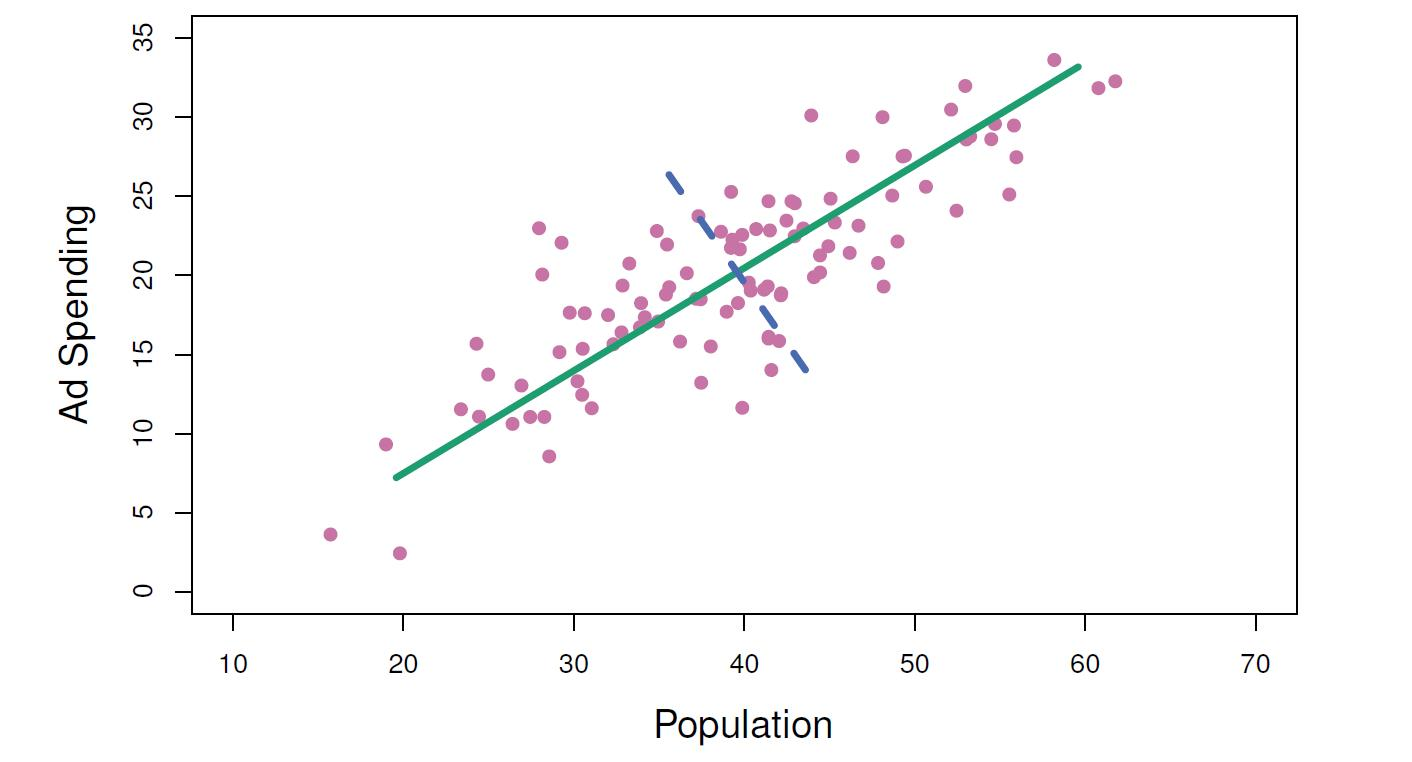
\includegraphics[scale=0.30]{IMG/PCAexample.jpg}
\end{figure}
\vspace{-0.5cm}
\centering Sample dataset with 2 variables. Green line indicates the first principal component, blue dashed line indicates $Z_2$.
\end{frame}
%---------------------------------------------------------------------
\begin{frame}{Principal component analysis (PCA)}
\vspace{-1.5cm}
\begin{figure}
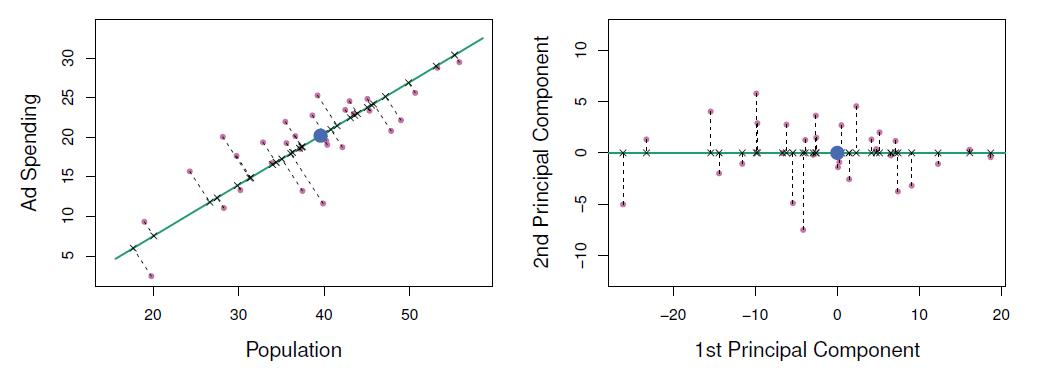
\includegraphics[scale=0.45]{IMG/PCAexample2.jpg}
\end{figure}
\vspace{-0.5cm}
\centering Sample dataset with 2 variables. Values of $z_{i1} \in Z_1$ and $z_{i2} \in Z_2$ are shown. Right panel/plot rotated for readability.
\end{frame}
%---------------------------------------------------------------------
\begin{frame}{Principal component analysis (PCA)}
\begin{itemize}
\item Constraining $Z_2$ to be uncorrelated with $Z_1$ is equivalent to constraining the direction $\bm{\phi}_2$ to be orthogonal (perpendicular) to the direction $\bm{\phi}_1$. 
\medskip
\item Subsequent principal components: \\ \medskip For a sequence of additional $Z_2, Z_3,\dots$ principal components, we solve \eqref{PCA1} while adding orthogonality condition with respect to all preceding principal components.
\medskip
\item Important geometrical interpretations to principal components apply (see \textcolor{blue}{\underline{\href{http://www-bcf.usc.edu/~gareth/ISL/}{ISLR textbook}}}).
\end{itemize}
\end{frame}
%---------------------------------------------------------------------
\begin{frame}{Principal component analysis (PCA)}
\textbf{Proportion of variance explained by principal components}\\
\begin{itemize}
\item To understand the ``strength'' of each principal component, we calculate the proportion of variance explained by each component.
\medskip
\item \textbf{Total variance present in a data set} (assuming centered variables with mean zero) is defined as:
$$ \sum_{j=1}^p \textit{var}\,(X_j) 
   = \sum_{j=1}^p \frac{1}{n} \sum_{i=1}^n x_{ij}^2 $$
\item \textbf{Variance explained} by the $m$-th principal component is:
$$ \textit{var}\,(Z_m) 
   = \frac{1}{n} \sum_{i=1}^n z_{im}^2 $$
\item $\sum_{j=1}^p \textit{var}\,(X_j) = \sum_{m=1}^M \textit{var}\,(Z_m), $  where $M = \min(n-1, p)$.
\end{itemize}
\end{frame}
%---------------------------------------------------------------------
\begin{frame}{Principal component analysis (PCA)}
\textbf{Proportion of variance explained (PVE)}\\
\bigskip
\begin{itemize}
\item PVE of the $m$-th principal component lies between 0 and 1 and it is defined as:
$$\textnormal{PVE}_m 
 = \frac{\sum_{i=1}^n z_{im}^2 }
 {\sum_{j=1}^p \sum_{i=1}^n x_{ij}^2}  $$\\
\bigskip
\item PVEs sum to 1. We can display \& interpret cumulative PVEs.
\end{itemize}
\end{frame}
%---------------------------------------------------------------------
\begin{frame}{Principal component analysis (PCA)}
\texttt{R} example:\\
\smallskip
\footnotesize{
\texttt{pca1 = princomp(x, scores=TRUE, cor=TRUE) \# x has 7 columns\\
summary(pca1)\\
~\\
\#\# Importance of components:\\
\#\# ~~~~~~~~~~~~~~~~~~~~~~~~~~Comp.1~~~~~Comp.2~~~~~Comp.3~~~~~~Comp.4\\
\#\# Standard deviation~~~~~1.9036937~ 1.0423367~ 0.81837919~ 0.75632747\\
\#\# Proportion of Variance 0.5177214~ 0.1552094~ 0.09567779~ 0.08171875\\
\#\# Cumulative Proportion~ 0.5177214~ 0.6729308~ 0.76860854~ 0.85032729\\
\#\# ~~~~~~~~~~~~~~~~~~~~~~~~~~Comp.5~~~~~~Comp.6~~~~~~Comp.7\\
\#\# Standard deviation~~~~~0.64958592~ 0.56978592~ 0.54871770\\
\#\# Proportion of Variance 0.06028027~ 0.04637943~ 0.04301302\\
\#\# Cumulative Proportion~ 0.91060756~ 0.95698698~ 1.00000000\\
}
\begin{itemize}
\item The number of components is also the number of variables.
\item Proportion of variance: Eg. if .85 then component explains 85\% of the variance.
\item Cumulative Proportion: $Z_m$ and previous components (adding up to 1).
\item Standard deviation = eigenvalues
\item How many components to use in PCR? Choose the components with eigenvalues equal or higher then 1. (or use cross-validation)
\end{itemize}
}
\end{frame}




%---------------------------------------------------------------------
\begin{frame}{Kaiser-Meyer-Olkin (KMO) statistic}
PCA can perform a compression of the available information (reduce dimension) only if we can ``reject''  independence (orthogonality) among variables.
\bigskip
Individual KMO (for $j$-th variable):
$$\textit{KMO}_j = \frac{\sum_{i\neq j} r_{ij}^2}{\sum_{i\neq j} r_{ij}^2 + \sum_{i\neq j} a_{ij}^2}\,;\hspace{1,7cm} \textit{KMO}_j \in \langle 0,1 \rangle $$\\
Overall KMO:
$$\textit{KMO} = \frac{\sum_j \sum_{i\neq j} r_{ij}^2}
                   {\sum_j \sum_{i\neq j} r_{ij}^2 \,+\, \sum_j \sum_{i\neq j} a_{ij}^2}\,
                   ;\hspace{0.5cm} \textit{KMO} \in \langle 0,1 \rangle $$\\

where:\\
$\{r_{ij} \} = \bm{R}$, which is a correlation matrix,\\
$\{a_{ij} \} = \bm{A}$, which is a partial correlation matrix\\
$a_{ij} = - \frac{v_{ij}}{\sqrt[]{v_{ii} \cdot v_{jj}\,}}$ where $\{ v_{ij} \} = \bm{V} = \bm{R}^{-1}$
\end{frame}
%------------------------------------------------
\begin{frame}{Kaiser-Meyer-Olkin (KMO) statistic}
KMO description 
\begin{itemize}
\item KMO compares  correlations between variables against their partial correlations. 
\item If partial correlations $a_{ij}$ are near zero, PCA can perform efficiently, because the
variables are highly related and KMO $\approx 1$.
\item If KMO is low (KMO $\approx 0$, often KMO $< 0.5$), PCA is not relevant.
\end{itemize}
\bigskip
KMO-based variable selection:
\smallskip
\begin{itemize}
\item Overall KMO should be .60 or higher (ideally over 0.90).
\item If it is not, drop the variables with the lowest individual KMO statistic values, until overall KMO rises above .60.
\item This approach requires that we start with multiple variables/regressors in our dataset; at least $p > 5$ .
\item KMO \& Bartlett’s test in \texttt{R}: \textcolor{blue}{\underline{\href{https://rstudio-pubs-static.s3.amazonaws.com/135029_f7211c7b041d4d69a67a09fcc482d82c.html}{see RStudio web page}}})
\end{itemize}
\end{frame}
%------------------------------------------------
\subsection{Principal component regression (PCR)}
\begin{frame}{Principal component regression (PCR)}

\textbf{PCR motivation:}\\
\bigskip
If we have many correlated original variables as regressors in a LRM, we can replace them with a small set of principal components that capture their joint variation.
\medskip
\begin{itemize}
\item Variance-Bias tradeoff benefits
\item Models unsuitable for LRM-like parameter interpretation
\end{itemize}
\end{frame}
%------------------------------------------------
\begin{frame}{Principal component regression (PCR)}
\begin{itemize}
\item Using PCA, we linearly transform our dataset of predictors $X_1, X_2, \dots, X_p$ into $Z_1, Z_2, \dots, Z_M$ variables where $M < p$. \\The PCA transformation can be outlined as follows: 
\begin{equation} \label{PCR1}
Z_m = \sum_{j=1}^p \phi_{mj} X_j,
\end{equation}
for some constant parameters $\phi_{m1}, \dots, \phi_{mp}$.
\item Now, we can use OLS to fit a LRM:
\begin{equation} \label{PCR2}
y_i = \theta_0 + \sum_{j=1}^M \theta_m z_{im} + \varepsilon_i,
\end{equation}
\item Note that in model \eqref{PCR2}, the regression coefficients are given
as $\theta_0, \dots, \theta_M$. If the constants $\phi_{m1}, \dots , \phi_{mp}$ are chosen wisely (PCA), then such dimension reduction approaches can often
outperform OLS regression in terms of CV errors, etc.
\end{itemize}
\end{frame}
%------------------------------------------------
\begin{frame}{Principal component regression (PCR)}

From equation/definition \eqref{PCR1}, we can write
$$ \sum_{m=1}^M \theta_m z_{im} 
= \sum_{m=1}^M \theta_m \sum_{j=1}^p \phi_{mj} x_{ij} 
= \sum_{j=1}^p \sum_{m=1}^M \theta_m \phi_{mj} x_{ij} 
= \sum_{j=1}^p \beta_j x_{ij} 
$$ 
where 
\begin{equation} \label{PCR3}
\beta_j = \sum_{m=1}^M \theta_m \phi_{mj}.
\end{equation}

\begin{itemize}
\item Therefore, model \eqref{PCR2} can be thought of as a special case of the original linear regression model.
\item Dimension reduction serves to constrain the estimated $\beta_j$ coefficients, since now they must take the form \eqref{PCR3}.
\item This approach can have significant benefits in terms of bias-variance tradeoff.
\end{itemize}
\end{frame}
%------------------------------------------------
\begin{frame}{Principal component regression (PCR)}
PCR: algorithm
\begin{itemize}
\medskip
\item First, we apply principal components analysis (PCA) to find suitable linear combinations of predictors for use in our regression.
\medskip
\item The first principal component is that (normalized) linear
combination of the regressors that has the largest variance.
\medskip
\item The second principal component has largest variance,
subject to being uncorrelated with the first.
\medskip
\item And so on. 
\medskip
\item The dependent variable is then regressed on few principal components, rather than many original regressors.\\ \medskip
The optimal number of principal components can be assessed using cross validation.
\end{itemize}
\bigskip

\end{frame}
%------------------------------------------------
\begin{frame}{Principal component regression (PCR)}
\vspace{-1cm}
\begin{figure}
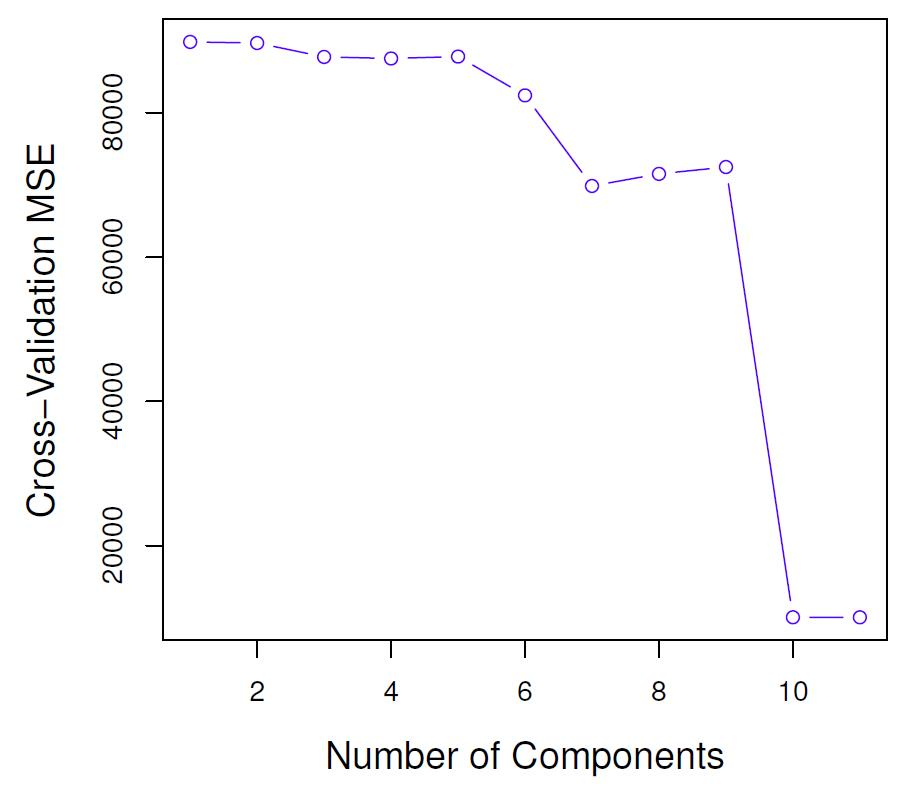
\includegraphics[scale=0.30]{IMG/PCRcomponent.jpg}
\end{figure}
\vspace{-0.5cm}
\centering Sample data, selection of the number of components.
\end{frame}
%------------------------------------------------
\begin{frame}{Principal component regression (PCR)}
\textbf{PCR: final discussion}
\medskip
\begin{itemize}
\item PCA identifies linear combinations (directions) that best
represent the predictors $X_1, X_2, \dots , X_p$.
\item These directions are identified in an \textbf{unsupervised} way, since the response $y$ is not used to help determine the principal component directions. i.e. the response does not supervise the identification of the principal components.
\item PCR suffers from a potentially serious drawback: there is no guarantee that the directions that best explain the predictors will also be the best directions to use for predicting the response.
\end{itemize}
\medskip
Potential solutions to the problem:
\begin{itemize}
\item Partial least squares (not covered here, see \textcolor{blue}{\underline{\href{http://www-bcf.usc.edu/~gareth/ISL/}{ISLR, ch. 10}}})
\end{itemize}
\end{frame}

%---------------------------------------------------------------------

\end{document}